Um mittels BLE ein Piconet zu bilden, ist ein Advertiser notwendig. Auf drei vorgegebenen Frequenzen, den Advertising Channels (siehe Sektion \ref{sec: le phy channel}), sendet er Daten, mit denen er sich für andere Geräte bemerkbar macht (Advertisements). Dabei können Advertisements auch genutzt werden, um Nutzdaten zu senden. Jedes Advertisement-Paket beinhaltet eine Bluetooth-Adresse des Senders, die 48 Bit lang ist.
\\\\
Geräte, die Daten auf den Advertising Channels empfangen, werden Scanner bzw. Initiator genannt. Auf diesem Weg finden sich die Geräte (Discovering). Der Initiator unterscheidet sich vom Scanner, da er in der Lage ist, sich zu einem Advertiser zu verbinden, von dem er ein Advertisement erhalten hat, das eine Verbindung ermöglicht. Sind zwei Geräte verbunden, senden und empfangen sie ihre Pakete auf den Data Channels (siehe Sektion \ref{sec: le phy channel}). Verbinden sich zwei Geräte, wird der Initiator als Master und der Advertiser als Slave angesehen.
\\\\
Durch die Anwendung von Zeitmultiplexing senden die Geräte ihre Pakete immer zu festgelegten Zeitpunkten. Dabei ist ein Event ein zeitlicher Abschnitt, in dem zusammenhängende Daten in Form von Paketen gesendet bzw. empfangen werden.

\begin{figure}[H]
    \centering
    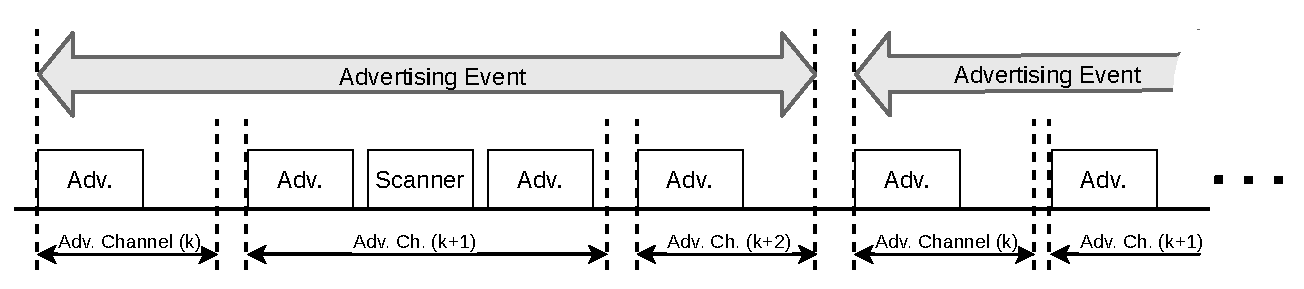
\includegraphics[width=\textwidth]{graphics/advertising_event.pdf}
    \caption[Advertising Event]{Advertising Event \cite{BtSpec4.0_127}}
    \label{fig: adv event}
\end{figure}
% QUELLE Spec S. 127 oben

In Abb. \ref{fig: adv event} ist ein Advertising Event dargestellt, bei dem ein Advertiser auf allen drei Advertising Channels nacheinander Advertisement-Pakete sendet. Auf dem zweiten Kanal empfängt der Advertiser -direkt im Anschluss auf sein erstes Advertisement-Paket- in diesem Kanal ein Paket eines Scanners, auf das er mit einem weiteren Advertisement antwortet.

\begin{figure}[H]
    \centering
    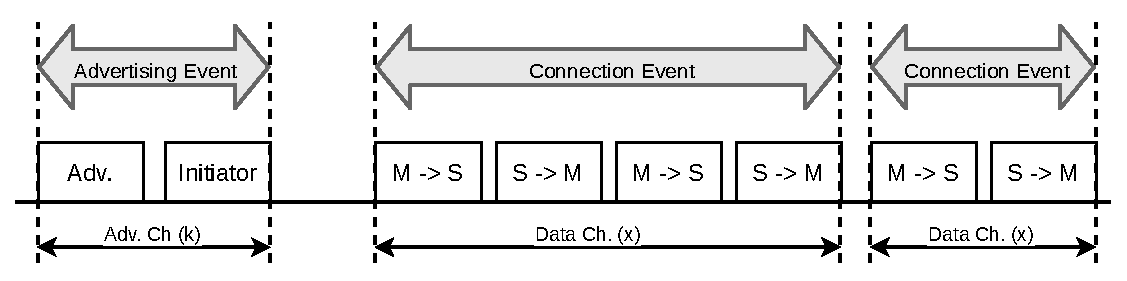
\includegraphics[width=0.9\textwidth]{graphics/advertising_initiator_event.pdf}
    \caption[Advertising und Connection Event]{Advertising und Connection Event \cite{BtSpec4.0_127}}
    \label{fig: adv init}
\end{figure}
% QUELLE Spec S. 127 unteres bild

In Abbildung \ref{fig: adv init} ist ein Advertising Event dargestellt, bei dem ein Initiator auf das Advertisement-Paket eines Advertiser antwortet, um eine Verbindung aufzubauen. Darauf folgt ein Connection Event, bei dem Master (ursprünglich Initiator) und Slave (ursprünglich Advertiser) einander Pakete auf einem Data Channel senden. Danach folgt ein weiteres Connection Event auf einem anderen Data Channel.